%% LaTeX-Beamer template for KIT design
%% by Erik Burger, Christian Hammer
%% title picture by Klaus Krogmann
%%
%% version 2.1
%%
%% mostly compatible to KIT corporate design v2.0
%% http://intranet.kit.edu/gestaltungsrichtlinien.php
%%
%% Problems, bugs and comments to
%% burger@kit.edu

\documentclass[18pt]{beamer}

%% SLIDE FORMAT

% use 'beamerthemekit' for standard 4:3 ratio
% for widescreen slides (16:9), use 'beamerthemekitwide'

\usepackage{templates/beamerthemekit}
% \usepackage{templates/beamerthemekitwide}

% \usepackage[dvips]{graphicx}
% \graphicspath{{pics/}}

%% TITLE PICTURE

% if a custom picture is to be used on the title page, copy it into the 'logos'
% directory, in the line below, replace 'mypicture' with the
% filename (without extension) and uncomment the following line
% (picture proportions: 63 : 20 for standard, 169 : 40 for wide
% *.eps format if you use latex+dvips+ps2pdf,
% *.jpg/*.png/*.pdf if you use pdflatex)

%\titleimage{mypicture}

%% TITLE LOGO

% for a custom logo on the front page, copy your file into the 'logos'
% directory, insert the filename in the line below and uncomment it

%\titlelogo{mylogo}
\titlelogo{empty_logo}

% (*.eps format if you use latex+dvips+ps2pdf,
% *.jpg/*.png/*.pdf if you use pdflatex)

%% TikZ INTEGRATION

% use these packages for PCM symbols and UML classes
% \usepackage{templates/tikzkit}
% \usepackage{templates/tikzuml}

% the presentation starts here

\title[Cosmic rays data center]{Current status of data center for cosmic rays \\based on KCDC}
\subtitle{GRID-2018, Dubna}
\author{Dmitriy Kostunin, Victoria Tokareva}

\institute{Institute for Nuclear Physics (IKP)}

\date{September 12, 2018}

% Bibliography

\usepackage[citestyle=authoryear,bibstyle=numeric,hyperref,backend=biber]{biblatex}
\addbibresource{templates/example.bib}
\bibhang1em

\newcommand{\itemarrow}{\scriptsize\raise1.25pt\hbox{\textcolor{kit-green100}{$\blacktriangleright$}}}
\newcommand{\concl}[1]{\item[\itemarrow]\textcolor{kit-green100}{#1}}
\renewcommand{\thefootnote}{\fnsymbol{footnote}}

\begin{document}

% change the following line to "ngerman" for German style date and logos
\selectlanguage{english}

%title page
\begin{frame}
\titlepage
\end{frame}

%table of contents
% \begin{frame}{Introduction}
% % Ориентировочный план действий:
% \begin{itemize}
%   \item Вводная:
%   \begin{itemize}
%     \item astroparticle physics и как это всё дофига важно
%     \item тренды: больше станций или общие данные?
%     \item итого: совместная российско-немецкая инцициатива
%   \end{itemize}
% \end{itemize}
% \end{frame}

\begin{frame}{Introduction: The secret life of the astroparticle data}
%или "Астрофизика - современное состояние"))
\small
\begin{columns}
  \begin{column}[t]{0.45\textwidth}
    \begin{center}
      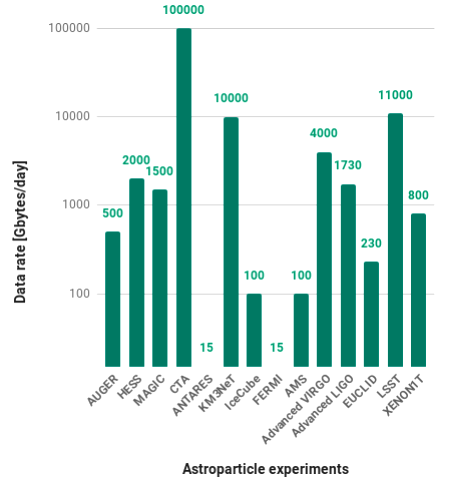
\includegraphics[width=0.79\linewidth]{pics/appec_base4.png}
    \end{center}
    \vspace{-2\parsep}
    \small Modern astroparticle experiments data rate [Gbytes/day]\footnotemark[1] %, source: APPEC brochure on Computing, 2016}
  \end{column}
  \hfill
  \begin{column}[t]{0.53\textwidth}
    % \vspace{1.5em}
    % Вступление - такие вступление :)
    % Современная астрофизика представлена большим количеством экспериментов, которые изучают примерно одно и то же (а зачастую - и прям совсем одно и то же, в плане объекта), но по-разному - т.е., в разных природных условиях и с использованием разных типов детекторов.
    % Каждый год данных прибывает, и при этом общй дата пул ежегодно растет, как на дрожжах (см. картинку)
    \begin{itemize}
    \item Wide range of experiments;
    \item Looking at the same sky with diffrent eyes: different detectors, different reactions under the study;
    \item Common data rate for astrophysical experiments all together is a few PBytes/yeary, which is comparable to the current LHC output\footnotemark[1] % \textcolor{red}{(ссылка на брощюру!!!)}
    \item Deep learning is coming...
    \item Need for collaboration
    \end{itemize}

%     \textcolor{red}{TODO: дописать текста, чтобы сбалансирвоать дизайн страницы}
  \end{column}
\end{columns}
  \footnotesize\footnotetext[1]{APPEC brochure on Computing, 2016}
\end{frame}

\begin{frame}{\textcolor{kit-green100}{KRAD}: \textcolor{kit-green100}{K}arlsruhe-\textcolor{kit-green100}{R}ussian \textcolor{kit-green100}{A}stroparticle \textcolor{kit-green100}{D}ata Life Cycle}
% \vspace{-1em     }
%     \begin{figure}[h]
\begin{center}
  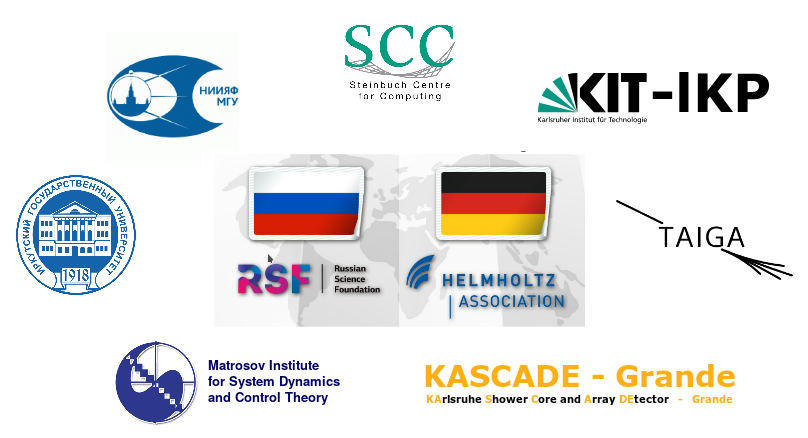
\includegraphics[width=0.9\linewidth]{pics/Collab.png}
\end{center}
\vspace{-2\parsep}
%     \caption{\small The frist Russian-German big data collaboration}
%     \label{ris:image}
%     \end{figure}
The first Russian-German big data collaboration

\end{frame}

\begin{frame}
Work packages:
\begin{itemize}
 \item Astroparticle data center (based on KCDC kcdc.ikp.kit.edu )
 \item Software for big data processing (“Data Life Cycle Lab”)
 \item Multimessenger data analysis
 \item Go for the public ( astroparticle.online )
\end{itemize}
% Как можно догадаться по названию, являет совместным Российско-немецким проектом, включающим в себя с российской стороны такие инстиутты как ... (перечислить, какие)
% Суть: создание единого центра обработки астрофизических данных.
\end{frame}

\begin{frame}{KASCADE}
\footnotesize
\begin{minipage}{0.69\textwidth}
  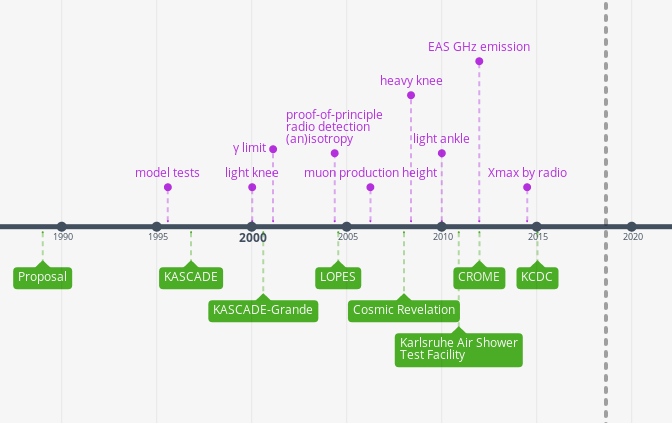
\includegraphics[width=1\textwidth,height=0.45\textheight]{pics/timeline_kascade.png}
\end{minipage}
\hfill
\begin{minipage}{0.29\textwidth}
  \begin{block}{Calorimeter}
    \begin{itemize}
      \setlength{\itemsep}{0pt}
      \item iron sampling
      \item liquid ionization chambers
      \item area 16m x 20m
      \item height 4.5m
    \end{itemize}
  \end{block}
\end{minipage}

\vspace{-1ex}
\begin{minipage}[t]{0.48\textwidth}
  \begin{block}{KASCADE}
    \begin{itemize}
      \setlength{\itemsep}{0pt}
      \item 200m x 200m field
      \item 252 detector stations
      \item station:
      \item[] ~--~$e$/$\gamma$ detectors (liquid scintillator)
      \item[] ~--~$\mu$ detector (plastic scintillator)
    \end{itemize}
  \end{block}
\end{minipage}
\hfill
\begin{minipage}[t]{0.48\textwidth}
  \begin{block}{GRANDE}
    \begin{itemize}
      \setlength{\itemsep}{0pt}
      \item 700m x 700m field
      \item 37 detector stations
      \item station:
      \item[] ~--~10m$^2$
      \item[] ~--~all-charged particle detector (16 plastic scintillators)
    \end{itemize}
  \end{block}
\end{minipage}
% \begin{center}
% \end{center}
% \vspace{-2\parsep}
%     \caption{\small The KASCADE experiment timeline}
% \textcolor{red}{Short descr.}
\end{frame}

\begin{frame}{TUNKA}
\footnotesize
\vspace{-2em}
\begin{minipage}[t]{0.48\textwidth}
  \begin{block}{Tunka-133}
    \centering
    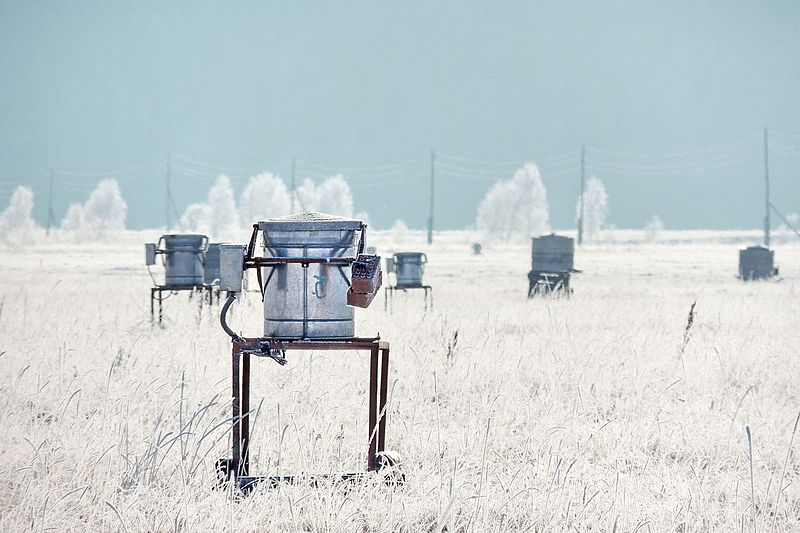
\includegraphics[height=0.23\textheight]{pics/Tunka-133.jpg}\vspace{-2ex}

    \begin{itemize}
      \setlength{\itemsep}{0pt}
      \item 133 photomultipliers
      \item measures EAS Cherenkov light
    \end{itemize}
  \end{block}
\end{minipage}
\hfill
\begin{minipage}[t]{0.48\textwidth}
  \begin{block}{Tunka-Rex}
    \centering
    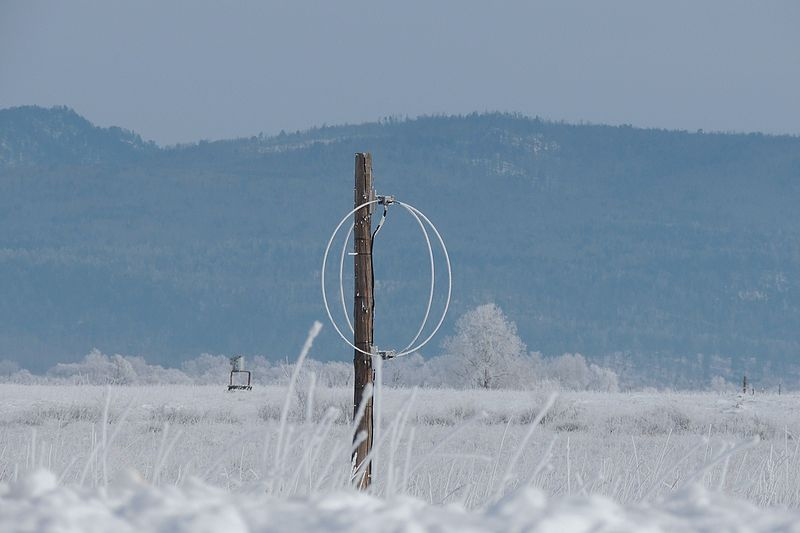
\includegraphics[height=0.23\textheight]{pics/Tunka-Rex.jpg}\vspace{-2ex}

    \begin{itemize}
      \setlength{\itemsep}{0pt}
      \item 63 antennas
      \item measures EAS radio-emission
    \end{itemize}
  \end{block}
\end{minipage}

\vspace{-1ex}
\begin{minipage}[t]{0.48\textwidth}
  \begin{block}{Tunka-Grande}
    \centering
    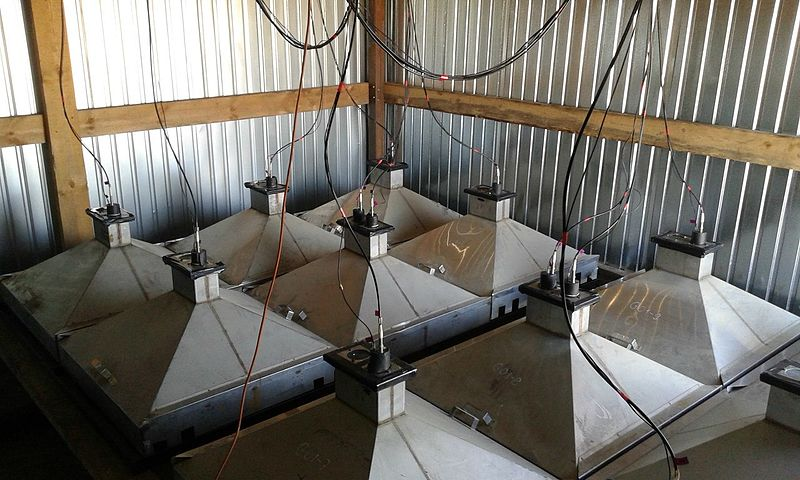
\includegraphics[height=0.23\textheight]{pics/Hiller_Roman-005.jpg}\vspace{-2ex}

    \begin{itemize}
      \setlength{\itemsep}{0pt}
      \item 380 scintillators 0.64m$^2$ each
      \item measures $e$/$\mu$ from EAS
    \end{itemize}
  \end{block}
\end{minipage}
\hfill
\begin{minipage}[t]{0.48\textwidth}
  \begin{block}{Tunka-HiSCORE}
    \centering
    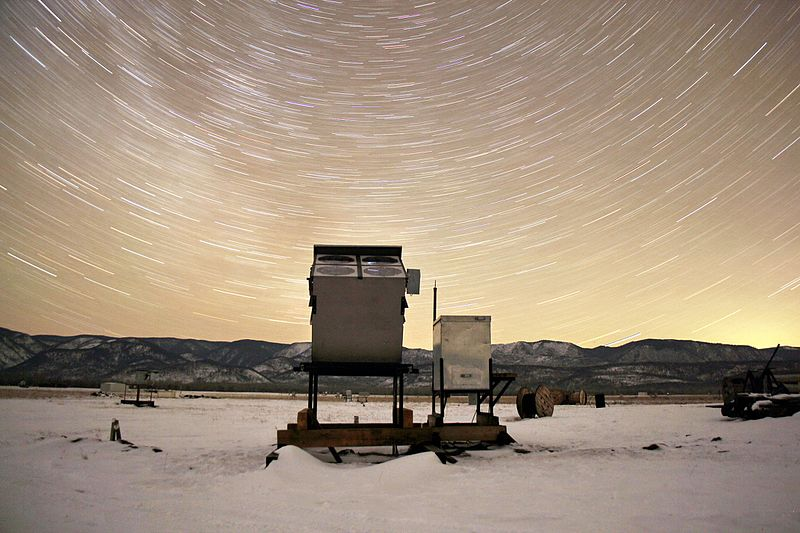
\includegraphics[height=0.23\textheight]{pics/Tunka-HiSCORE.jpg}\vspace{-2ex}

    \begin{itemize}
      \setlength{\itemsep}{0pt}
      \item 47 photomultipliers
      \item measures EAS Cherenkov light
    \end{itemize}
  \end{block}
\end{minipage}


\end{frame}

% \begin{frame}[allowframebreaks]{Outline}
% \begin{itemize}
%  \item сравнение KASCADE и Tunka (почему должно быть интересно объединить данные, проблемы и решения):
%  %обязательно сказать, что в астрофизике такое делается вперые (хотя в целом тема не нова), и мы работаем в столрону proof of work
%  \begin{itemize}
%     \item физика: в чем разница собираемых данных?
%     \item разница по метаданным
%     \item организация хранения: у KASCADE есть KCDC, и всё крайне аккурктно оргинизовано (рассказать, как),
%     у Tunka все в процессе (оказывается, есть крутой слайд у Костюнина про это (5/13))
%     \item обработка? общая она или раздельная? в чем разница? как мошла бы выглядеть общая схема обработки?
%     \item как можно было бы организовать совместный быстрый доступ пользователей к данным/инструментам анализа?
%     \item почему мы считаем, что эксперименты можно определить, и почему именно Tunka()?
%  \end{itemize}
%  \item Как мы думаем, это можно было бы сделать:
%     \begin{itemize}
%         \item MWS как идея
%         %при объединении распрд. ресурсов возникает такое понятие, как интероперабельность системы. она может быть обеспечена на 3-х уровнях: организационном (т.е., руками), техническом (автоматизация процессов)  и семантическом
%         \item какие-нибудь схематические догадки о том, как это все касается нас
%         \item job workflow
%         \item какую систему будем юзать?
% \end{itemize}
% \item А что уже сделанно к наст моменту?
%     \begin{itemize}
%      \item общая схема KCDC
%      \item astroparticle.online
%      \item описание метаданных
%     \end{itemize}
% \item Conclusion: мы собрались делать большое дело, у нас есть богатая история, много планов и даже чуть-чуть из них уже сделано. Следующим шагом проекта станет...
% % \tableofcontents
% \end{itemize}
%
% \end{frame}

\begin{frame}{?? TITLE ??}
\begin{columns}
  \begin{column}[t]{0.49\textwidth}
    \begin{block}{Different}
      \begin{itemize}
        \item Data format (depends on avalilable detectors)
        \item Information on detector properties (e.g.\ calibrations)
        \item Dedicated software for analyzing data
        \item Sometimes: special system environment for the software
        \item \textcolor{red!50!black}{Currently}: separate APIs and user interfaces for different experiments
      \end{itemize}
    \end{block}
  \end{column}
  \hfill
  \begin{column}[t]{0.49\textwidth}
    \begin{block}{Common}
      \begin{itemize}
        \item Metadata format (e.g.\ time, location, atmospheric conditions)
        \item Software for EAS simulation (e.g. KORSIKA)
        \item Shower parameters
        \item Theoretical models
        \item \textcolor{blue!50!black}{Bright future}: unified API and user interface for different experiments
      \end{itemize}
    \end{block}
  \end{column}
\end{columns}
\end{frame}

\begin{frame}{What is WMS?}
\textcolor{red}{\textit{Taken from Petrosyan's talk}}
\begin{itemize}
  \item WMS~--- workload management system
  \item Providing a central queue for all users, makes hundreds of distributed sites appear as local
  \item Hide middleware while supporting diversity and evolution
  \begin{itemize}
    \item WMS interacts with middleware, users see only high level workflow
    \item Automation engines built in WMS, not exposed to users
  \end{itemize}
  \item Hide variations in infrastructure
  \begin{itemize}
    \item WMS presents uniform ‘job’ slots to user
    \item Easy to integrate grid sites, clouds, HPC sites
  \end{itemize}
  \item Use the same system for simulation, data processing and users analysis
  \item Similar ideas have been implemented in several independent systems developed by LHC experiments: AliEn, Dirac, PanDA
\end{itemize}
\end{frame}

\begin{frame}{Data storage}
\begin{tabular*}{1\textwidth}{p{0.45\textwidth}@{\extracolsep{\fill}}p{0.45\textwidth}}
\hline\multicolumn{2}{c}{Location} \\
Experiments: remote locations with no or limited internet access &
Servers: data are transferred periodically on tapes or disks \\
\hline\multicolumn{2}{c}{Data} \\
Raw detector readouts: analyzed offline, not stored &
Pre-analyzed events: stored on servers \\
\hline\multicolumn{2}{c}{Different \& common} \\
Each experiment has its own detectors and provides its own format of events &
Events share \emph{common metadata} (e.g.\ time, location, atmospheric conditions) \\
\hline\multicolumn{2}{c}{Storage} \\
It is proposed to store unique event id and metadata in the unified database &
With growing data sizes, distribured storage for events could be useful \\
\hline
\end{tabular*}
\end{frame}

\begin{frame}{Data storage}
\begin{itemize}
  \item Some experiments (in our case, TUNKA) are situated at remote locations with no or limited internet access, raw data are transferred periodically to servers on tapes or disks
  \item Raw data are pre-analyzed, so-called ``direct'' observables ($e$, $\mu$, $\gamma$, $\hat{C}$, radio, etc.) are obtained, events are stored on servers
  \item Each experiment has its own detectors and provides its own format of events
  \item Events share \emph{common metadata} (e.g.\ time, location, atmospheric conditions)
  \item It is proposed to store unique event id and metadata in the unified database
  \item With growing data sizes, distribured storage for events could be useful
\end{itemize}
\end{frame}

\begin{frame}{Proposed cosmic-ray metadata structure}
\vspace{-1.5em}
\begin{center}
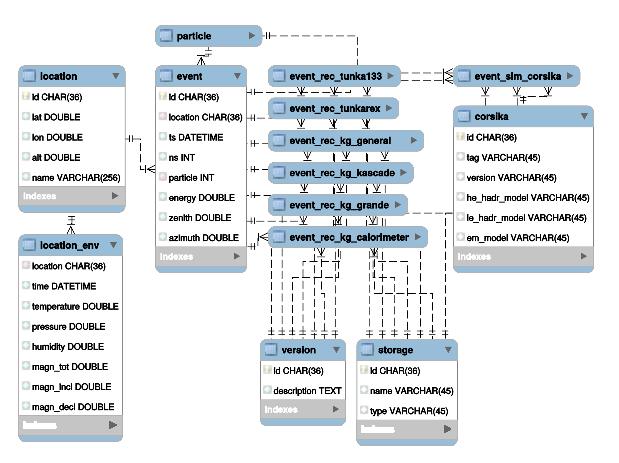
\includegraphics[width=0.82\textwidth]{pics/metadata.eps}
\end{center}
\end{frame}

\begin{frame}{Data analysis}
\begin{itemize}
  \item Software for data analysis depends on a particular experiment
  \begin{itemize}
    \item It may even require dedicated system environment
  \end{itemize}
  \concl{Virtualization could be useful}
  \item Data analysis requires huge amounts of input data
  \begin{itemize}
    \item It is often more optimal to perform it on the same site the data are stored
  \end{itemize}
  \concl{Job management could handle the task}
\end{itemize}
\end{frame}

\begin{frame}{Simulation}
\begin{itemize}
  \item The software for EAS simulation (e.g.\ KORSIKA) does not depend on a particular experiment
  \concl{Simulations require standartized system environment}
  \item Simulations require small amounts of input data
  \item Simulations can be done independently for different events
  \concl{Simulations are easily scalable}
  \item Simulations require a lot of computing resources
  \concl{Conclusion: distributed computing could be useful}
\end{itemize}
\end{frame}

\begin{frame}{Mapping of observables between experiments}
\textcolor{red}{We need to write something here}

\textcolor{red}{We could look at Kostunin's slide \#8}

\begin{block}{Draft}
  \begin{itemize}
    \item Calibrations provided by experiments
    \item Various models
    \item Implementations are stored
  \end{itemize}
\end{block}
% \begin{center}
%   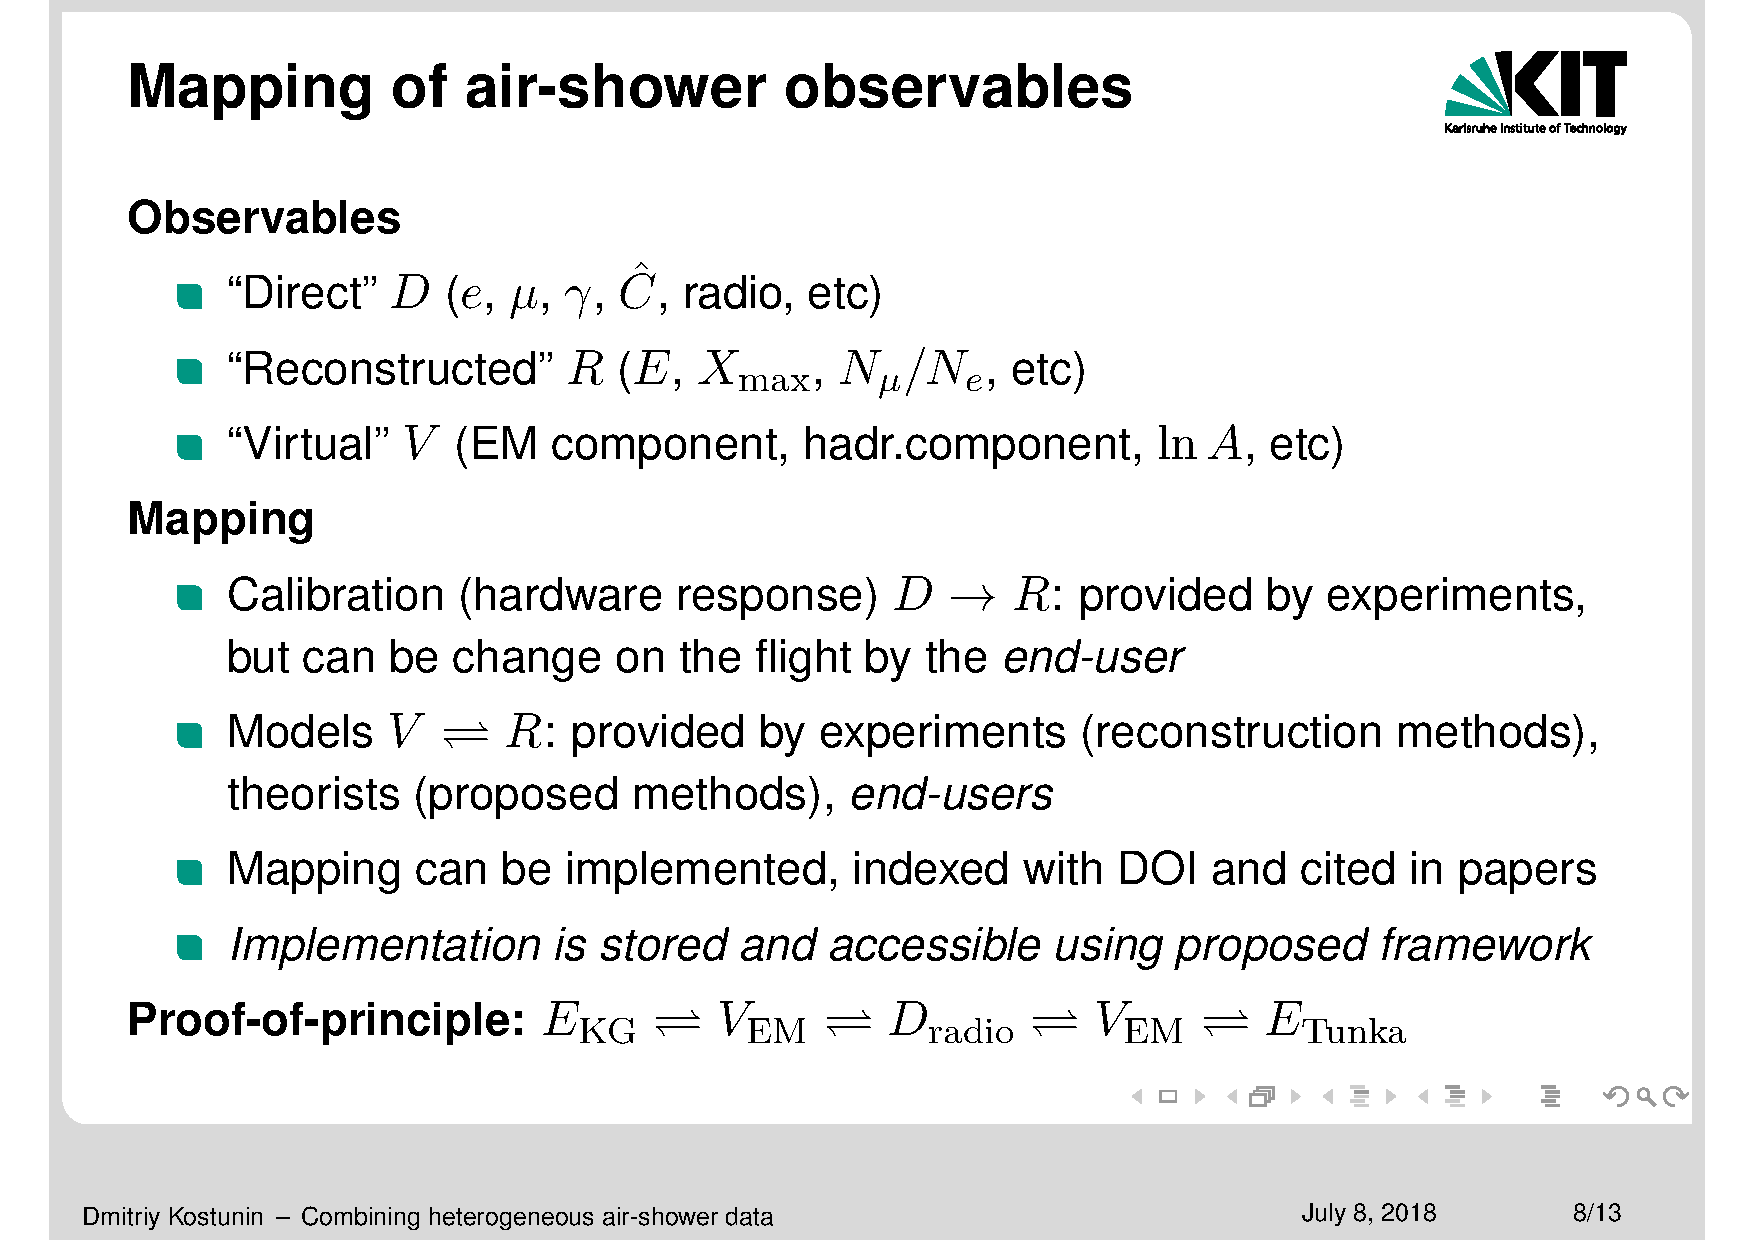
\includegraphics[width=0.7\textwidth]{pics/k8.pdf}
% \end{center}
\end{frame}

\begin{frame}{Access}
\begin{block}{Draft}
  \begin{itemize}
    \item Benefits of open access
    \item Education and outreach
    \item Which infrastructure to use?
  \end{itemize}
\end{block}
\end{frame}

\begin{frame}{Distributed analisys scheme}
% \textcolor{red}{Схема~--- проверить!)}
\begin{center}
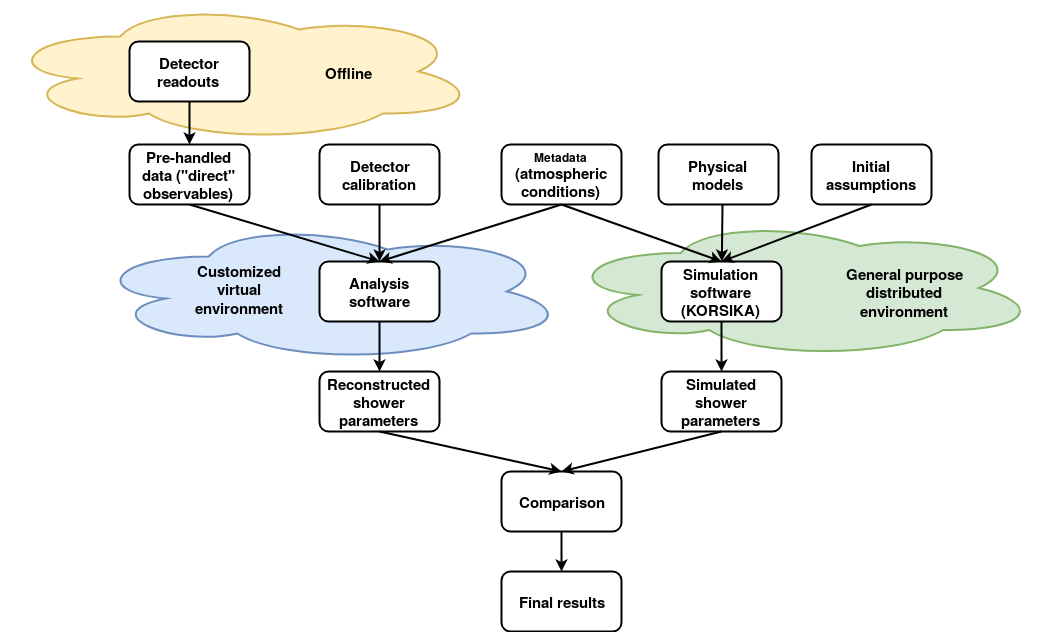
\includegraphics[width=0.85\textwidth]{pics/KCDC_workflow_f1.png}
\end{center}
\end{frame}

\begin{frame}{Current status and outlook}
\begin{block}{And what has already been done so far?}
  \begin{itemize}
    \item KCDC general scheme
    \item astroparticle.online
    \item metadata description
  \end{itemize}
\end{block}
\begin{block}{Conclusion}
  \begin{itemize}
    \item We are going to do a great job, we have a rich history, many plans and even a few of them have already been done. The next step of the project will be\ldots
  \end{itemize}
\end{block}
\end{frame}

\begin{frame}{TODO}
\textcolor{red}{What else is missing?}
\end{frame}

\begin{frame}{}
\Huge
\begin{center}
\textcolor{kit-green100}{Thank you\\for your attention!}

\vspace{1em}
\Large
% \textcolor{kit-green100}{
Any questions?
% }
\end{center}
\end{frame}

%
% \begin{frame}{test}
%  \begin{columns}
% \begin{column}[t]{5cm}
%     text1
% \end{column}
%
% \begin{column}[t]{5cm}
% text2
% \end{column}
% \end{columns}
% \end{frame}


% \section{Section 1}
% \subsection{Subsection 1.1}
% \begin{frame}{Example slide A}
% \begin{itemize}
% \item PCM, Citation: \cite{becker2008a} %\language
% \pause
% \item Bullet point 2
% \item \dots
% \end{itemize}
% \end{frame}
%
% \subsection{Subsection 1.2}
% \begin{frame}{Example slide B}
% \begin{block}{Block 1}
% \begin{itemize}
% \item Bullet point 1
% \pause
% \item Bullet point 2
% \item \dots
% \end{itemize}
% \end{block}
% \end{frame}
%
% \section{Section 2}
% \begin{frame}{Example slide C}
% \begin{exampleblock}{Example 1}
% \begin{itemize}
% \item Bullet point 1
% \pause
% \item Bullet point 2
% \item \dots
% \end{itemize}
% \end{exampleblock}
% \end{frame}
%
% \begin{frame}{Example slide D}
% \begin{alertblock}{Alert 1}
% \begin{itemize}
% \item Bullet point 1
% \pause
% \item Bullet point 2
% \item \dots
% \end{itemize}
% \end{alertblock}
% \end{frame}
%
% \appendix
% \beginbackup
%
% \begin{frame}[allowframebreaks]{References}
% \printbibliography
% \end{frame}
%
% \backupend

\end{document}
